\documentclass[tikz,border=10pt]{standalone}
\usepackage[T1]{fontenc}
\usepackage{mathpazo}
\usepackage{amsmath,amssymb}
\usetikzlibrary{arrows.meta, positioning, calc, patterns}

\definecolor{stblue}{HTML}{7B97AD}
\definecolor{rwgold}{HTML}{B8995E}
\definecolor{sage}{HTML}{7A9A7E}
\definecolor{dkbrown}{HTML}{3D3530}
\definecolor{wmgray}{HTML}{7B7067}
\definecolor{cream}{HTML}{F9F6F0}
\definecolor{border}{HTML}{D4C9B8}
\definecolor{terracotta}{HTML}{C47A6A}

\begin{document}
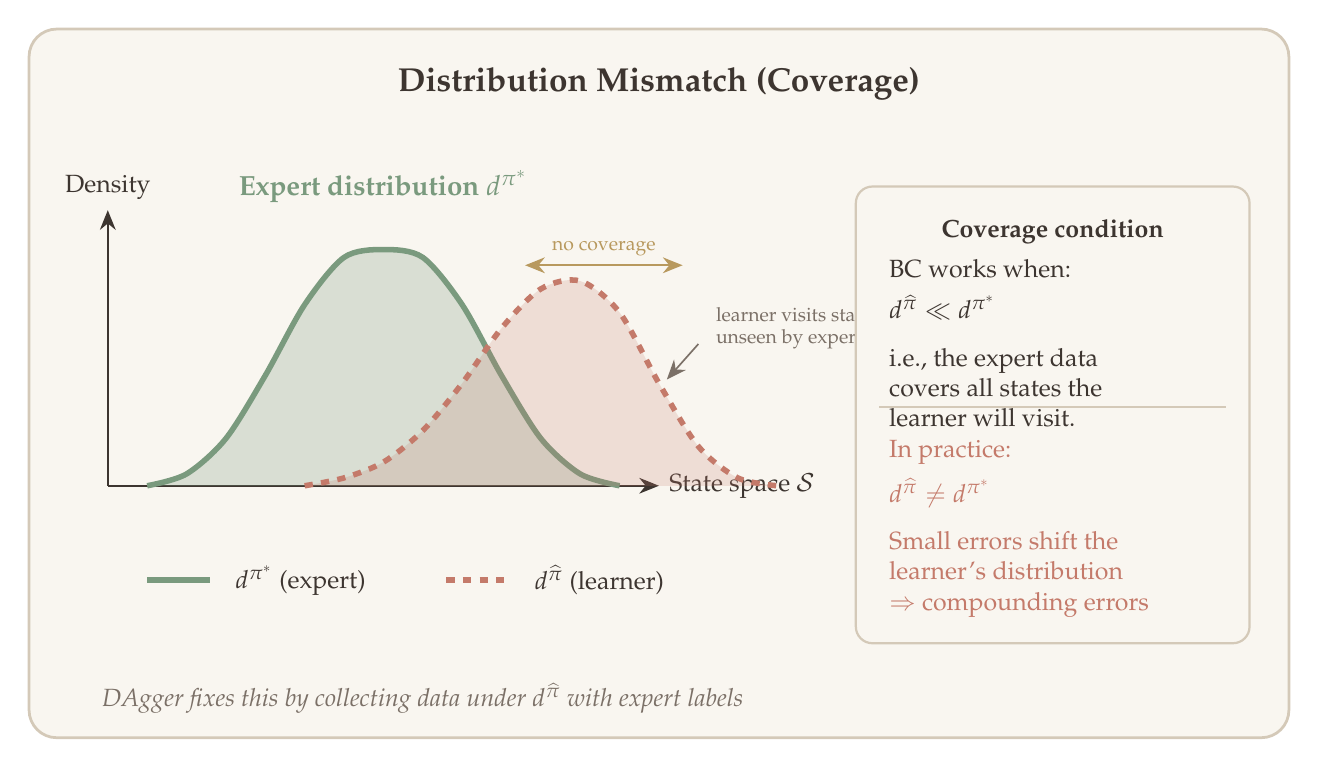
\begin{tikzpicture}[
  >={Stealth[length=2.5mm, width=2mm]},
]

% Background
\fill[cream, rounded corners=10pt] (-1.5,-3.2) rectangle (14.5,5.8);
\draw[border, rounded corners=10pt, line width=1pt] (-1.5,-3.2) rectangle (14.5,5.8);

% Title
\node[font=\large\bfseries, text=dkbrown] at (6.5,5.1)
  {Distribution Mismatch (Coverage)};

% ========================================
% Left panel: Expert distribution
% ========================================
\node[font=\normalsize\bfseries, text=sage] at (3.0,3.8) {Expert distribution $d^{\pi^*}$};

% Axes
\draw[->, line width=0.8pt, dkbrown] (-0.5,0) -- (6.5,0)
  node[right, font=\small] {State space $\mathcal{S}$};
\draw[->, line width=0.8pt, dkbrown] (-0.5,0) -- (-0.5,3.5)
  node[above, font=\small] {Density};

% Expert distribution (bell curve, centered)
\fill[sage, opacity=0.25] plot[smooth, tension=0.5] coordinates {
  (0.0, 0.0)
  (0.5, 0.15)
  (1.0, 0.6)
  (1.5, 1.4)
  (2.0, 2.3)
  (2.5, 2.9)
  (3.0, 3.0)
  (3.5, 2.9)
  (4.0, 2.3)
  (4.5, 1.4)
  (5.0, 0.6)
  (5.5, 0.15)
  (6.0, 0.0)
} -- cycle;

\draw[sage, line width=2pt, smooth, tension=0.5]
  plot coordinates {
    (0.0, 0.0)
    (0.5, 0.15)
    (1.0, 0.6)
    (1.5, 1.4)
    (2.0, 2.3)
    (2.5, 2.9)
    (3.0, 3.0)
    (3.5, 2.9)
    (4.0, 2.3)
    (4.5, 1.4)
    (5.0, 0.6)
    (5.5, 0.15)
    (6.0, 0.0)
  };

% Learner distribution (shifted right, less overlap)
\fill[terracotta, opacity=0.2] plot[smooth, tension=0.5] coordinates {
  (2.0, 0.0)
  (2.5, 0.1)
  (3.0, 0.3)
  (3.5, 0.7)
  (4.0, 1.3)
  (4.5, 2.0)
  (5.0, 2.5)
  (5.5, 2.6)
  (6.0, 2.2)
  (6.5, 1.3)
  (7.0, 0.5)
  (7.5, 0.1)
  (8.0, 0.0)
} -- cycle;

\draw[terracotta, line width=2pt, smooth, tension=0.5, dashed]
  plot coordinates {
    (2.0, 0.0)
    (2.5, 0.1)
    (3.0, 0.3)
    (3.5, 0.7)
    (4.0, 1.3)
    (4.5, 2.0)
    (5.0, 2.5)
    (5.5, 2.6)
    (6.0, 2.2)
    (6.5, 1.3)
    (7.0, 0.5)
    (7.5, 0.1)
    (8.0, 0.0)
  };

% Legend
\draw[sage, line width=2pt] (0.0,-1.2) -- (0.8,-1.2);
\node[font=\small, text=dkbrown, anchor=west] at (1.0,-1.2) {$d^{\pi^*}$ (expert)};

\draw[terracotta, line width=2pt, dashed] (3.8,-1.2) -- (4.6,-1.2);
\node[font=\small, text=dkbrown, anchor=west] at (4.8,-1.2) {$d^{\widehat\pi}$ (learner)};

% Overlap region annotation
\draw[rwgold, line width=0.8pt, <->] (4.8,2.8) -- (6.8,2.8);
\node[font=\scriptsize, text=rwgold, above] at (5.8,2.8) {no coverage};

% Gap annotation with brace
\draw[wmgray, line width=0.6pt, ->] (7.0,1.8) -- (6.6,1.35);
\node[font=\scriptsize, text=wmgray, anchor=west, align=left] at (7.1,2.0)
  {learner visits states\\unseen by expert};

% ========================================
% Right panel: Summary box
% ========================================
\draw[border, line width=0.8pt, rounded corners=6pt, fill=cream]
  (9.0,-2.0) rectangle (14.0,3.8);

\node[font=\small\bfseries, text=dkbrown, anchor=north] at (11.5,3.5)
  {Coverage condition};

\node[font=\small, text=dkbrown, align=left, anchor=north west] at (9.3,3.0) {%
  BC works when:\\[4pt]
  $d^{\widehat\pi} \ll d^{\pi^*}$\\[6pt]
  i.e., the expert data\\
  covers all states the\\
  learner will visit.
};

\draw[border, line width=0.5pt] (9.3,1.0) -- (13.7,1.0);

\node[font=\small, text=terracotta, align=left, anchor=north west] at (9.3,0.7) {%
  In practice:\\[4pt]
  $d^{\widehat\pi} \neq d^{\pi^*}$\\[6pt]
  Small errors shift the\\
  learner's distribution\\
  $\Rightarrow$ compounding errors
};

% Bottom annotation
\node[font=\small\itshape, text=wmgray, align=center] at (3.5,-2.7)
  {DAgger fixes this by collecting data under $d^{\widehat\pi}$ with expert labels};

\end{tikzpicture}
\end{document}
